\subsection{Folded Focus}\label{a: sink\source}
For the folded focus, we will consider an approach from fluid mechanics. This is to enable the reader to consider the dynamics within a different field with the aim to give more intuition in a fast-slow dynamical system. To aid with this concept one should consider the motion of water in a bathtub, when the plug has been removed. We can immediately observe that the water will start to spiral around the plug - much like Figure \ref{fig: spiral} - which acts in a similar fashion to the following figure. 
\begin{figure}[h!]
	\centering
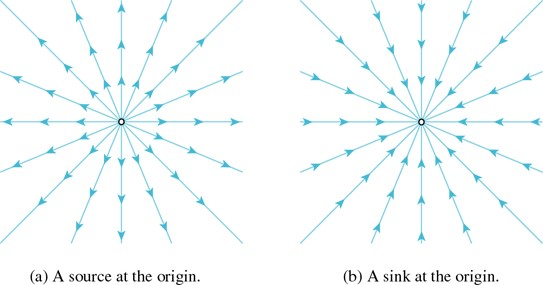
\includegraphics[width=0.7\linewidth]{Images/sourcesink}
	\caption{Oversimplified phase plane for a folded focus.}
	\label{fig:source-sink}
\end{figure}
From Figure \ref{fig:source-sink} we see that on the left we have a source within the system, by this we can observe that a source attracts the flow in the system. Whereas on the right we have a sink which can be seen to be repelling the flow, resulting in the jumps (Figure \ref{fig: vdp flow diagram}) or oscillation in the system - see Sections \ref{sec:singularitiesandfoldpoints} and \ref{sec: MMO Oscilaltions}. 